
%    Historical notes on the development of particle accelerators 
%        Late 1800s -> Cathode Ray Tubes  
%        1920s -> Electrostatic devices based on large potential difference
%        1930s -> Rolf Widerow and Ising LINAC alternating current accleration, limited by low frequency RF generators 
%        1930-1950 -> Cyclotrons and synchotrons 
%        1945-1955 -> WW2 technological increases in RF generation mean LINAC is again viable
%        1952 -> 1 GeV electron LINAC contructed at Stanford using 21 kylstron generators 

%
%  -------- Discovery of Mesons ---------
%	1934 - Yukawa theory of strong force w/ meson exchange 
%	1937 - Two groups looking at cosmics identify Yukawas meson (middle weight) (Anderson)
%	1947 - Kaons in cloud chambers
%	1950 - Lambda baryon (Anderson @CalTech)
%	1952 - Brookhaven Cosmotron begins operating as first modern accelerator and many particles discovered
%	1953 - Gell-Mann & Nishijima "strangeness"
%	1961 - Murray Gell-Mann, The eightfold way of organizing baryons and mesons by charge and strangeness
%	1964 - GM and Zweig do the quark model uds and it is great 


% Bjorken Scaling - Structure functions F1 and F2 are only mildly dependent on Q2.
% SLAC 5-20 GeV electron experiments 
%	% Predicted by the parton model 
% 

%	Updated Outline (May 2, 2019)
%		1. The Hof 
%		2. Quarks 
%		3. DIS and SFs 
%		4. Parton Model and PDFs 
%		5. HERA
%		6. SIDIS and SFs 
%		7. TMDs & Connections to SFs
%		8. This Measurement 
%		9. Unpolarized and BSA 
%		10. Wes

\chapter{Introduction}

%\begin{figure}
%	\centering
%	\label{fig:meson-octet}
%	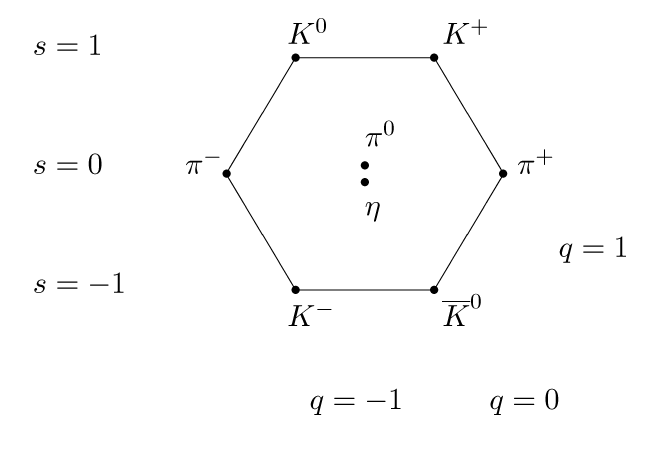
\includegraphics[width = \textwidth]{image/diagrams/meson_octet.png}	
%	\caption{}{}
%\end{figure}

% 1. The Hof 
%Prior to 1955 scientists thought that the proton was a point-like particle (having mass, but no spatial extent).  This became a testable hypothesis in 1952 with the ability to accelerate electrons up to 1 GeV using the Stanford "Mark III".  Theoretical tools of the day were sufficiently advanced to predict what the electron-proton scattering cross section should be, assuming that they interact electromagnetically as point particles \cite{history-rosenbluth:1950}.  That year Hofstadter and McAllister setup an experiment to collide electrons between 100-200MeV into stationary protons in their laboratory in Stanford, California and their findings would create the field of nucleon structure research, a field that remains very active today \cite{history-hofstadter:1955, history-hofstadter:1956, history-chambers:1956}.  Hoftstader observed a significant deviation of the cross section from that predicted Rosenbluth cross section.  We now know that Hofstadter was observing the scattering of electrons from the charged quarks which compose it, and discovering that the proton is not a point-like fundamental particle.

Research into the internal structure of protons and neutrons began in 1955 with the pioneering work of Hofstadter and McAllister.  Working together at Standford, the pair measured the electron-proton scattering cross section with 188 MeV electrons incident on hydrogen. Their measured cross section was inconsistent with the cross section predicted for a point-like proton, demonstrating its finite size.  Simultaneously, the Brookhaven Cosmotron produced an overwhelming number of new particles, creating what was dubbed a "particle zoo".  Theoretical efforts by Gell-Mann and Zwieg showed that the particle zoo could be explained by combinations of fractionally charged particles that Gell-Mann coined quarks.  

%	\begin{figure}
%		\centering
%		\label{fig:hofstadter}
%		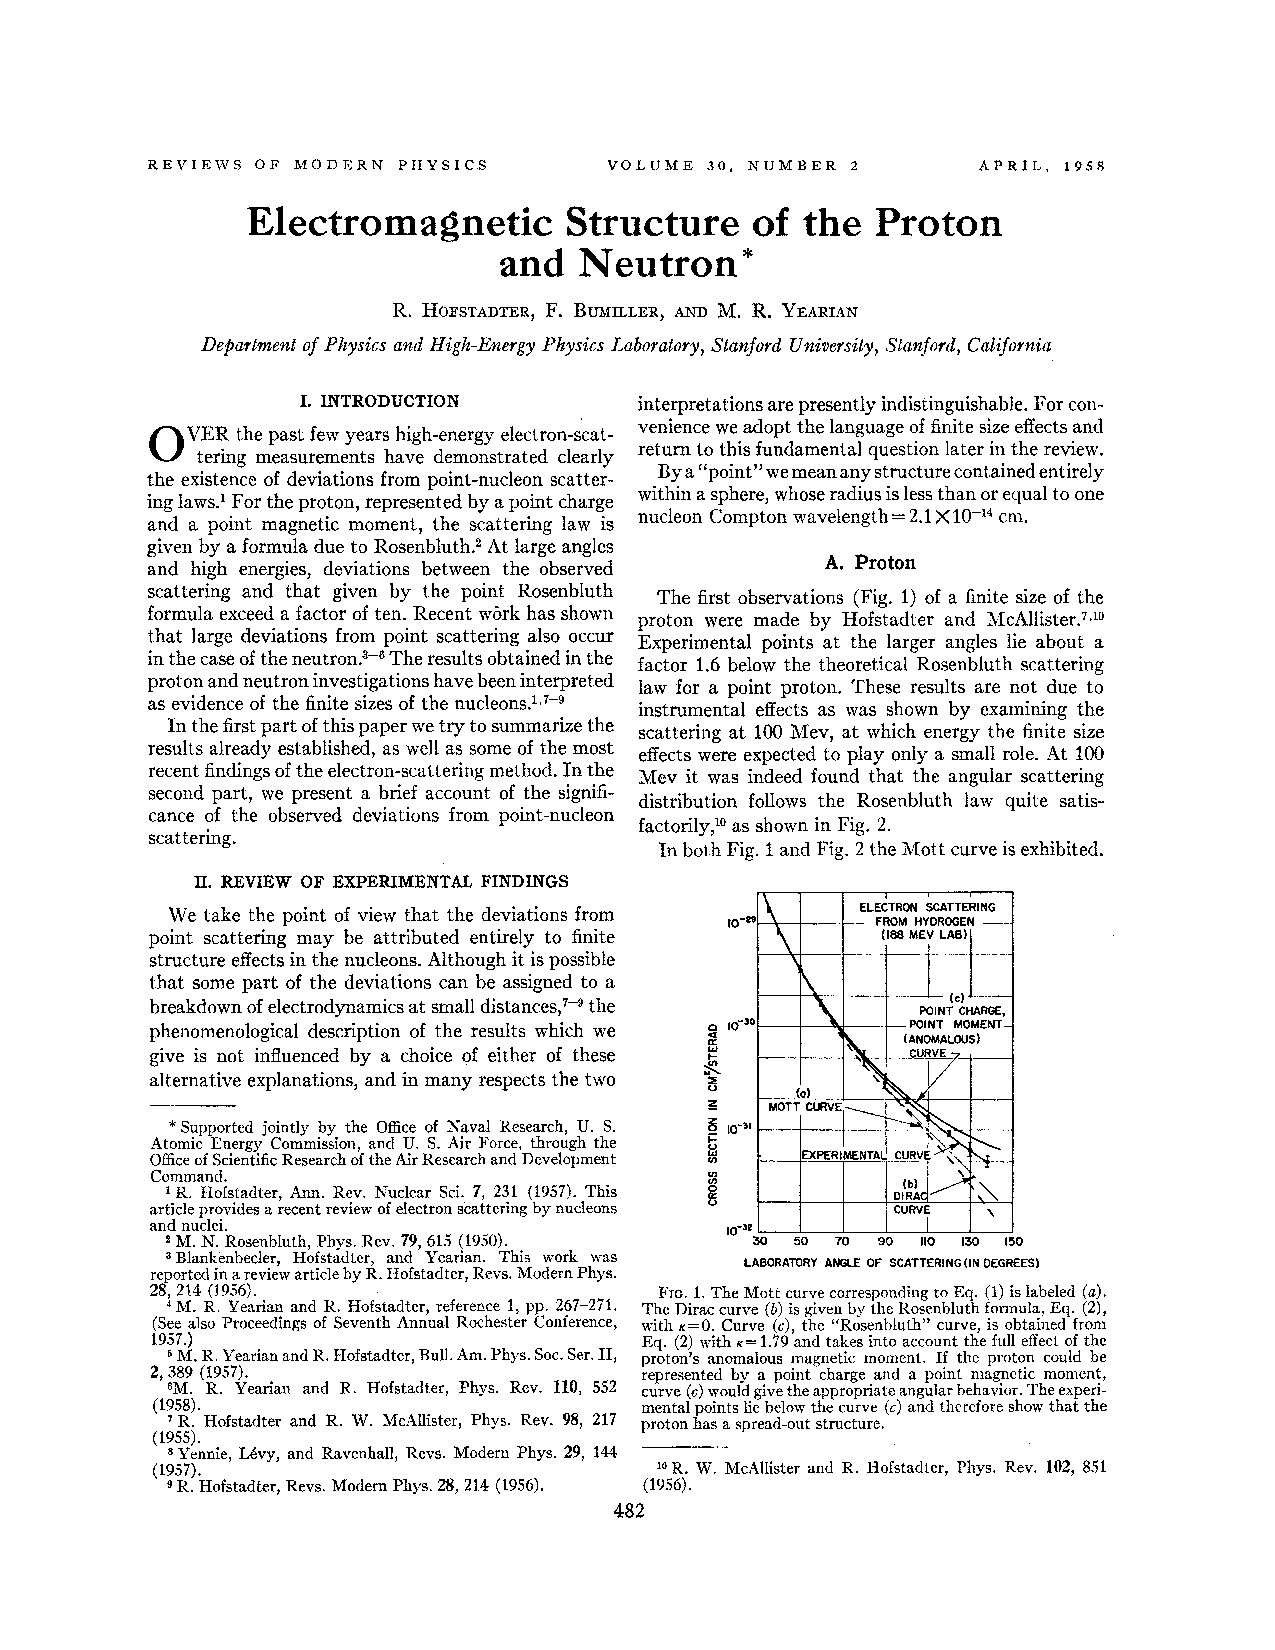
\includegraphics[width = \textwidth]{image/plots/introduction/hofstadter.pdf}	
%		\caption[Hofstadter and McAllister show that high energy electron proton scattering does not follow Rosenbluth formula.]{Hofstadter and McAllister results of scattering 188 MeV electrons from protons.  The results shown as black points disagree with predictions based on a point-like proton.  This plot motivated physicists to assert a finite size proton, and eventually study its substructure in terms of quarks and gluons.}	
%	\end{figure}

%\begin{equation}
%	\label{eqn:rosenbluth}
%	\frac{d\sigma}{d\Omega} = \frac{\alpha^2}{4 E_{1}^{2} sin^4(\theta/2)} \frac{E_3}{E_1} \left( \frac{G_{E}^2 + \tau G_{M}^2}{1 + \tau} cos^2(\theta/2) + 2 \tau G_{M}^2sin^2(\theta/2) \right)
%\end{equation}
%
%Where $\tau = \frac{Q^2}{4m_{p}^2}$.

%The Hofstadter results left physicists with a clear conclusion, the proton isn't point-like. To develop a hypothesis that explained what type of particle or particles protons and neutrons are made of would take ten years of further experimentation.  During that time particle accelerators increased in energy, until collisions became so energetic that new particles were produced.  At first, physicists interpreted this "particle zoo" as all new fundamental particles.  In 1966 Murray Gell-Mann and Somebody Somewhere explained this proliferation of particles as combinations of three more fundamental particles.  The idea that a complicated set of observed particles could be reduced to a simpler basis set of fundamental particles introduced a welcome simplification, but also introduced fractionally charged particles. Despite the large volume of scattering experiments taking place, fractionally charged particles had never been detected, and still haven't today.  The conclusion was that these new "quarks" are never found alone, but always in pairs or groups.

% 3. DIS and SFs
\section{Deeply Inelastic Scattering and Structure Functions}
%	Experiments in which an electron collides with a stationary proton at very high energies (much more than the mass of the proton) called deeply inelastic scattering (DIS) experiments began at the Stanford Linear Accelerator in 1966 shortly after the machine was commissioned.  The cross section from deeply inelastic electron-proton scattering can be parametrized in terms of two structure functions ($F_1(x, Q^2)$ $F2(x,Q^2)$).  By comparing the parton model cross section to this parametrization, the structure functions can be related to the PDFs.  Interestingly, the parton model implies that both $F_1$ and $F_2$ should be independent of $Q^2$.  This prediction came to be known as Bjorken scaling, and when it was observed in the early 1970s at SLAC confidence in the parton model picture swelled.

\begin{figure}
	\centering
	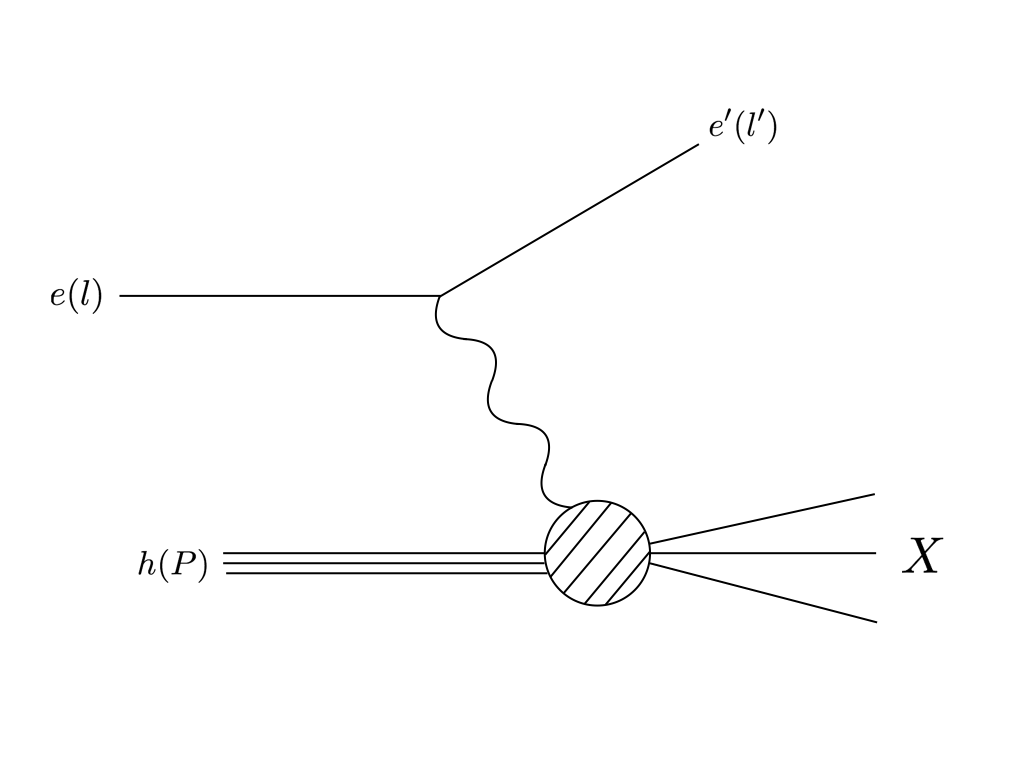
\includegraphics[width = \textwidth]{image/diagrams/dis-feynman.png}	
	\caption[A diagrammatic representation of deeply inelastic scattering.]{Deeply inelastic scattering (DIS) between a lepton and a hadron, in this thesis an electron and a proton.}
	\label{fig:dis}
\end{figure}

Learning more about quarks required scattering at higher energies.  As the incident energy of electrons in scattering experiments grows much larger than the proton mass, the inelastic scattering cross section dominates (electron kinetic energy is not conserved).  A \textit{deeply} inelastic scattering (DIS) event occurs when an electron collides with the target particle and transfers sufficient energy to interrogate it on a distance scale much smaller than its radius.  The cross section for DIS can be described in terms of two structure functions $F_1$ and $F_2$.  As we will see below, these structure functions describe quark momentum in the proton.

\begin{equation}
	\label{eqn:sfs}
	\frac{d^2\sigma}{dx dQ^2} = \frac{4 \pi \alpha^2}{Q^4} \left\lbrace \left( 1 - y - \frac{m_p^2 y^2}{Q^2} \right) \frac{F_2(x,Q^2)}{x} + y^2 F_1 (x,Q^2) \right\rbrace
\end{equation}

The electron kinematics are described by the four momentum transfer $q^{\mu} = l^{\mu} - l'^{\mu}$ (shown in figure \ref{fig:dis}), the negative momentum transfer $Q^2 = - q^{\mu} q_{\mu}$ and,
\begin{align}  
  x = \frac{Q^{2}}{2P \cdot q} && y = \frac{P \cdot q}{P \cdot l} 
\end{align}

where $x$ is called the momentum fraction and $y$ is the inelasticity.  The variable $x$ (which will appear throughout this thesis) is bound between zero and one and describes the fraction of the total proton momentum carried by the quark struck in the scattering.  For the case that $Q^2 \gg m_p^2 y^2$ the cross section can be approximated as shown below.

\begin{equation}
	\label{eqn:sfs2}
	\frac{d^2\sigma}{dx dQ^2} \approx \frac{4 \pi \alpha^2}{Q^4} \left\lbrace \left( 1 - y \right) \frac{F_2(x,Q^2)}{x} + y^2 F_1 (x,Q^2) \right\rbrace
\end{equation}

First measurements of the DIS structure functions \cite{history-bjorken:1969} showed that they are approximately independent of $Q^2$ (Bjorken scaling) and that they appear to be related to each other through the Callan-Gross relation \ref{eqn:callan-gross}.

\begin{equation}	
	F_{2} (x) = 2xF_1 (x)
	\label{eqn:callan-gross}
\end{equation}

Both of these features are predicted by the parton model, a tool introduced by Richard Feynman in 1969 \cite{history-feynman:1969}.

\section{The Parton Model and Parton Distribution Functions}
%Feynman's parton model stated that during high energy electron-proton collisions the electron enters with so much energy that the quarks which compose the proton are essentially stationary, and the electron simply scatters off of one part (quark or gluon) of the nucleus.  This "parton" model assumed that the cross section for electron-proton scattering was the product of an elastic scattering between a charged electron and quark (calculable using techniques from quantum electrodynamics), and a function that describes the momentum of the quark in the proton prior to the collision, called the parton distribution function (PDF).  Parton distribution functions are indexed with the variable $x$ that represents the fractional proton momentum carried by the struck quark.  

Feynman noted that high energy electron-proton collisions exist on a very short timescale, and can be imagined as electrons interacting electromagnetically (or electroweakly) with single quarks in the proton.  Elastic electron-quark scattering is calculable, but since the quark is not truly free a parton distribution function $q_i(x)$ was introduced to model the quarks interaction with the other constituents of the proton (the index $i$ refers to the quark flavor).  Simply put, the parton distribution functions (PDFs) describe the probability of finding a quark of flavor $i$ in a proton (or other hadron) with momentum fraction $x$ (this interpretation is no longer valid once the $Q^2$ evolution is calculated using DGLAP).  By using the parton model the DIS cross section can be predicted in terms of the PDFs.    

\begin{equation}
	\label{eqn:sfs-pdf}
	\frac{d^2\sigma}{dx dQ^2} = \frac{4 \pi \alpha^2}{Q^4} \left\lbrace 1 - y + \frac{y^2}{2} \right\rbrace \sum_{i} Q_i^2 q_i^p (x)
\end{equation}

When equating \ref{eqn:sfs2} with \ref{eqn:sfs-pdf} Bjorken scaling and the Callan-Gross relation are shown theoretically.

\begin{equation}
	\label{eqn:bjorken-scaling}
	F_{2} (x, Q^2) = 2xF_1 (x, Q^2) = x \sum_{i} Q_i^2 q_i^p(x)
\end{equation}

These first triumphs of the parton model lead to in depth studies of the structure functions at HERA.

\section{HERA}

% Most epic figure that exists in all of 
% nucleon structure research.
\begin{figure}
	\centering
	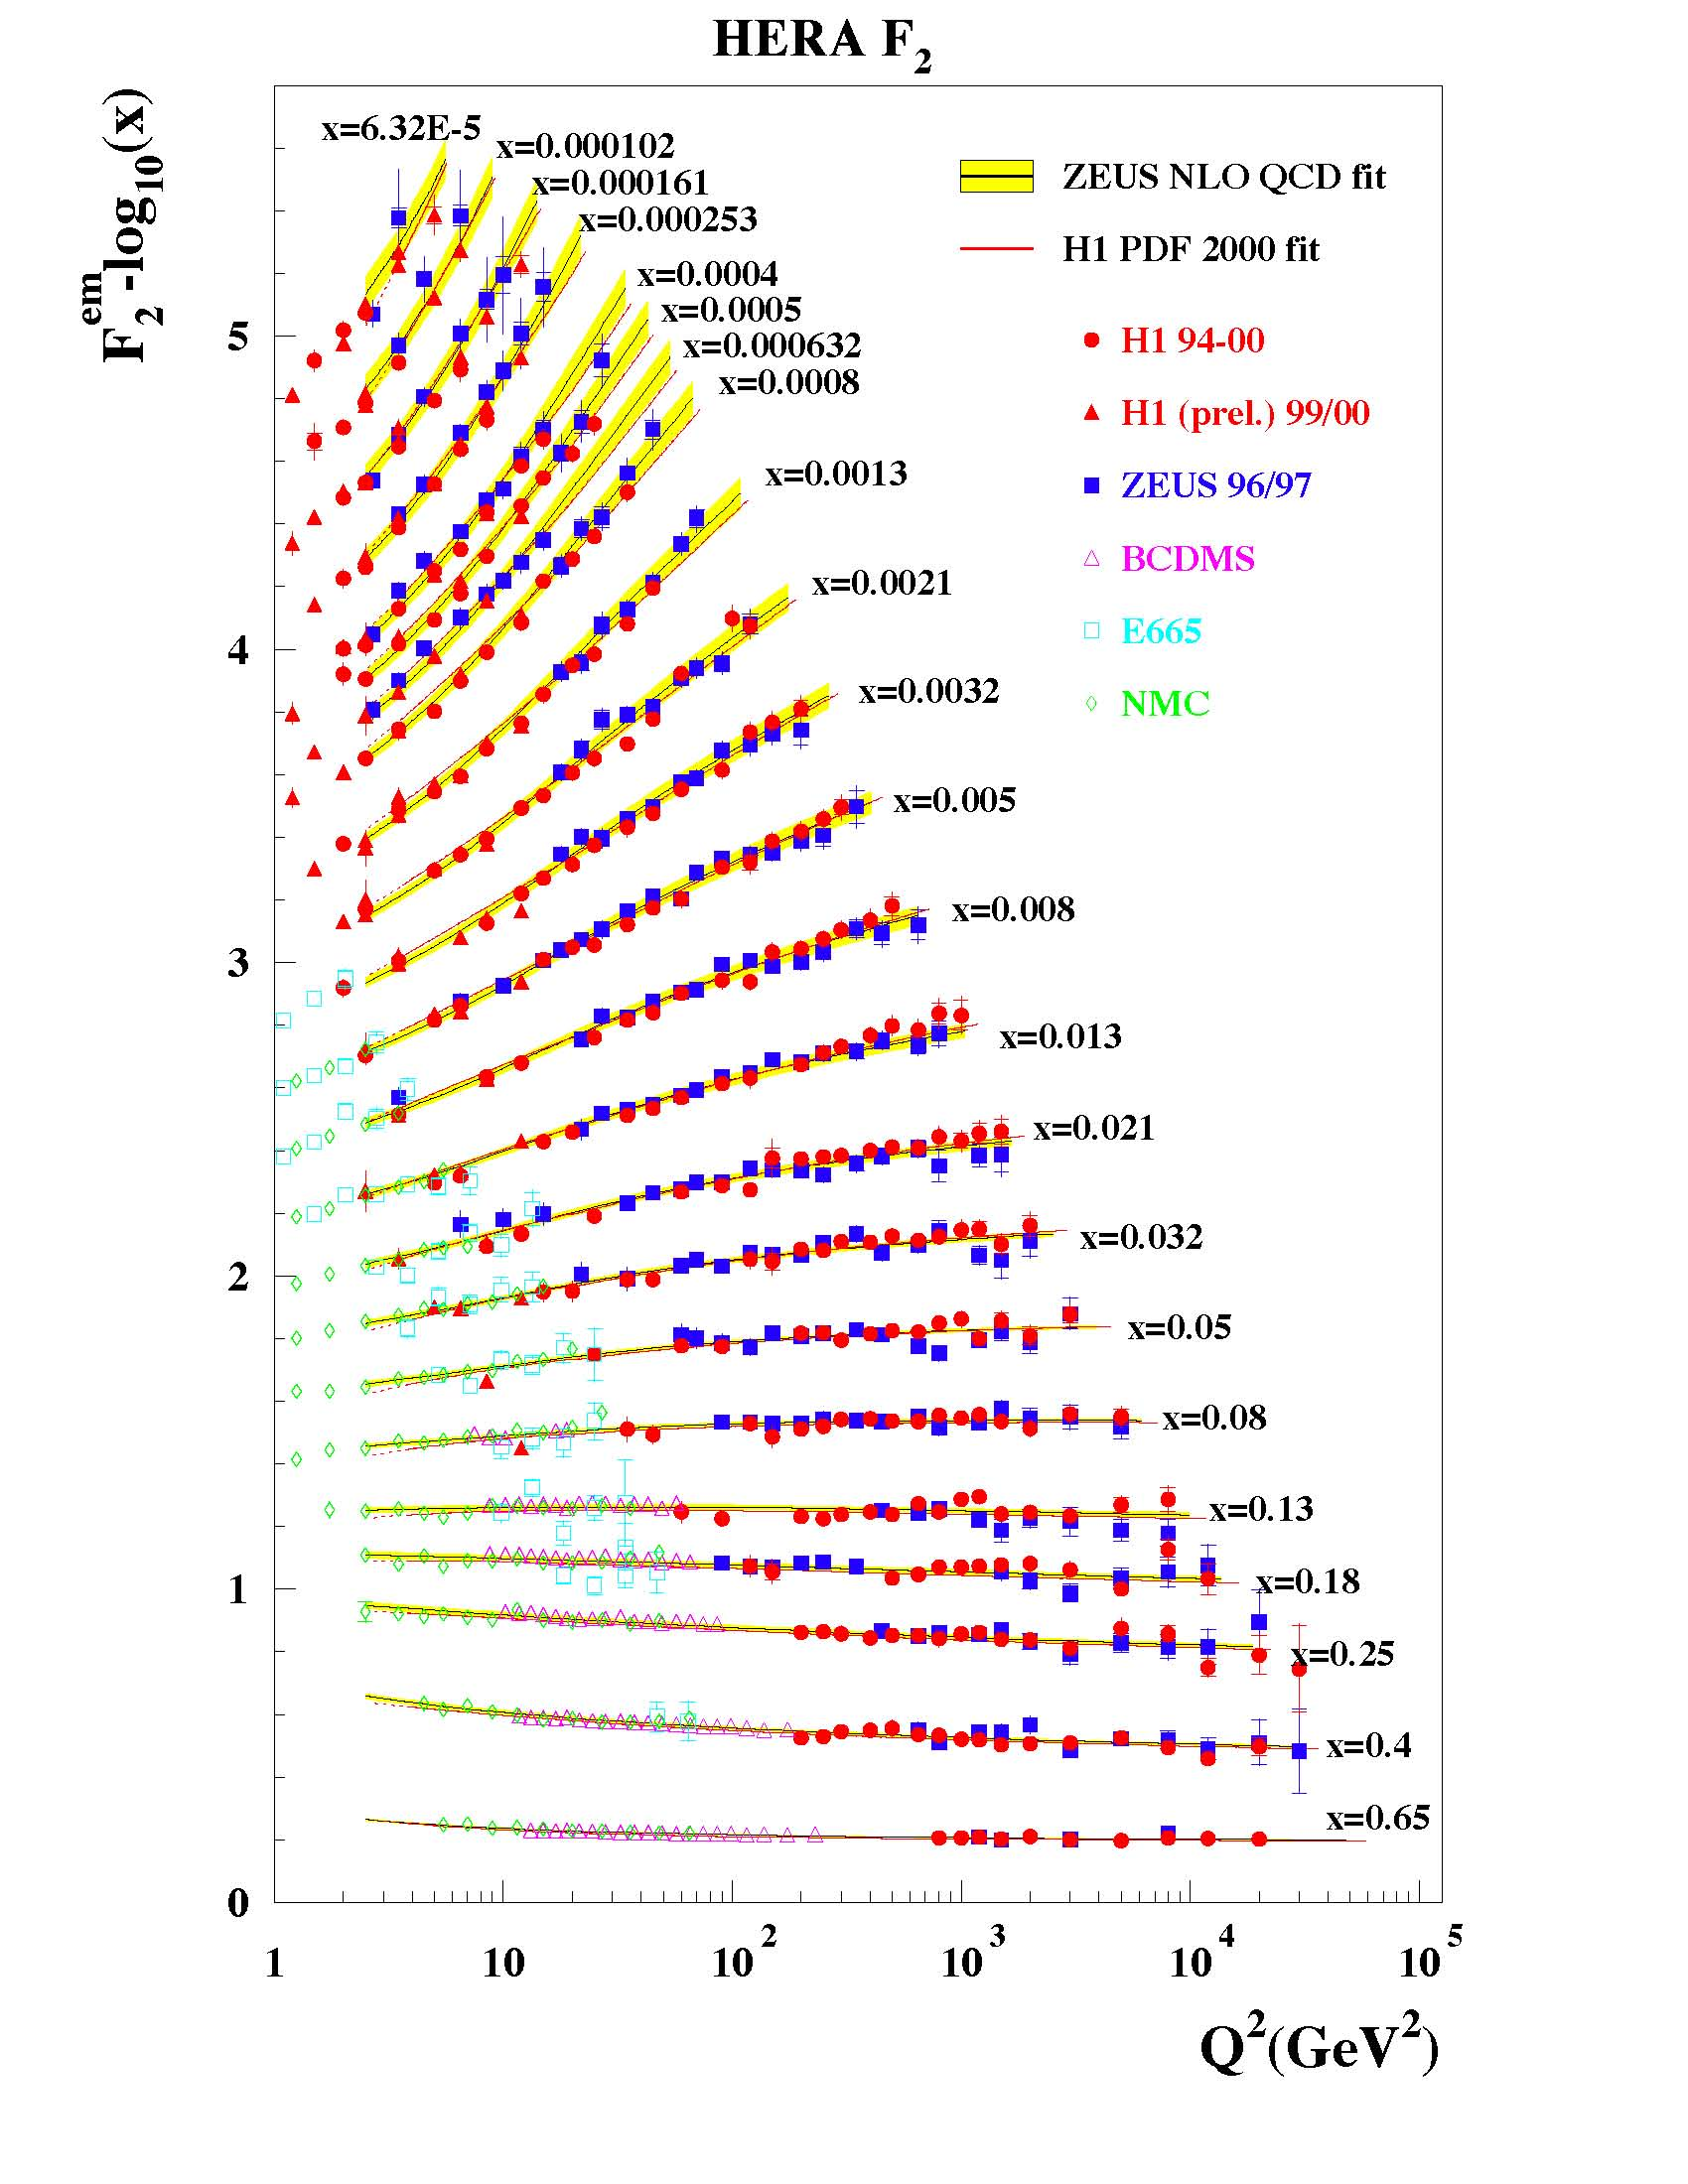
\includegraphics[width = \textwidth]{image/plots/introduction/f2.jpg}	
	\caption[$F_{2} (Q^2)$ results from HERA]{HERA experiments ZEUS and H1 mapped out the structure function $F_2$, which displayed the predicted Bjorken scaling for most values of $x$.   The mild $Q^2$ dependence of the PDFs can be calculated using the DGLAP evolution equations for the PDFs, providing an understanding for the observed dependence.}
	\label{fig:f2}
\end{figure}

HERA studied DIS extensively at large $Q^2 > 200 \; GeV^2$ by colliding 27.5 GeV electrons and 820 or 920 GeV protons.  The H1 and ZEUS experiments mapped proton structure functions in great detail.  The results \ref{fig:f2} display a weak dependence on $Q^2$; a feature calculable using the DGLAP evolution equations.  The PDFs extracted from these structure functions show that almost half of the proton momentum is carried by gluons (and quark/anti-quark pairs).  These results demonstrated that a simple picture of the proton as three valence quarks $(uud)$ is not sufficient.    

\section{Semi-Inclusive Deeply Inelastic Scattering}
DIS events where one hadron is detected in the final state are called semi-inclusive DIS (SIDIS) events.  The detection of a hadron in the final state provides the information needed to go beyond a discussion of quark momentum along the hard scattering direction and into the plane transverse to it.  A diagrammatic representation of the reaction \ref{fig:sidis} shows the hadron scattering out of the electron/virtual photon plane with angle $\phi$, also noted $\phi_h$ in other places.

\begin{figure}
	\centering
	\label{fig:sidis}
	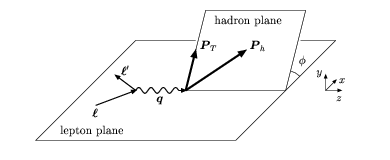
\includegraphics[width = \textwidth]{image/diagrams/phi-hadron.png}	
	\caption[Diagrammatic representation of SIDIS with hadronic $\phi_h$ angle.]{In a SIDIS event the scattered electron is detected as well as one final state hadron, allowing for the calculation of the angle $\phi_h$ which appears frequently in the SIDIS cross section.}
\end{figure}

Analogously to the manner in which the DIS cross section can be described by structure functions, the SIDIS cross section \ref{e:crossmaster} can be decomposed into a set of 18 structure functions (depending on the polarization direction of the electron and proton) \cite{tmds-mulders:1995}, \cite{tmds-bacchetta:2006}. 

\begin{eqnarray}
\frac{d\sigma}{dx_B \, dy\, d\phi_s \,dz\, d\phi_h\, d p_{h\perp}^2}
&=&\frac{\alpha^2_{em}}{2x_B y Q^2}
\frac{y^2}{1-\varepsilon}  ( 1+\frac{\gamma^2}{2x_B} ) \Bigl\{  \nonumber \\
&& F_{UU ,T} +  \varepsilon F_{UU ,L}
+ \sqrt{2\,\varepsilon (1+\varepsilon)} \cos\phi_h F_{UU}^{\cos\phi_h}
+ \varepsilon \cos(2\phi_h) F_{UU}^{\cos 2\phi_h} \nonumber \\
&+& \lambda_e
\sqrt{2\,\varepsilon (1-\varepsilon)} \sin\phi_h F_{LU}^{\sin\phi_h}
+ \lambda \big[ \sqrt{2 \varepsilon (1+\varepsilon)} \sin\phi_h F_{UL}^{\sin\phi_h}
  +  \varepsilon \sin(2\phi_h) F_{UL}^{\sin 2\phi_h} \big] \nonumber \\
&+&  \lambda_e \lambda
\big[\sqrt{1-\varepsilon^2} F_{LL}
  +\sqrt{2\varepsilon (1-\varepsilon)} \cos\phi_h F_{LL}^{\cos \phi_h}\big] \nonumber \\
&+& s_\perp
\big[ \sin(\phi_h-\phi_S) \bigl(F_{UT ,T}^{\sin(\phi_h -\phi_S)}
  + \varepsilon\, F_{UT ,L}^{\sin(\phi_h -\phi_S)}\bigr) \nonumber \\
  && \phantom{s_\perp}
  + \varepsilon \sin(\phi_h+\phi_S) F_{UT}^{\sin(\phi_h +\phi_S)}
  + \varepsilon \sin(3\phi_h-\phi_S) F_{UT}^{\sin(3\phi_h -\phi_S)} \nonumber \\
  && \phantom{s_\perp}
  + \sqrt{2\,\varepsilon (1+\varepsilon)} \sin\phi_S F_{UT}^{\sin \phi_S }
  + \sqrt{2\,\varepsilon (1+\varepsilon)} \sin(2\phi_h-\phi_S) F_{UT}^{\sin(2\phi_h -\phi_S)}\big]\nonumber \\
&+& \lambda_e s_\perp
\big[\sqrt{1-\varepsilon^2} \cos(\phi_h-\phi_S) F_{LT}^{\cos(\phi_h -\phi_S)}
  +\sqrt{2\varepsilon (1-\varepsilon)} \cos\phi_S F_{LT}^{\cos \phi_S} \nonumber \\
  && \phantom{\lambda_e s_\perp}
  +\sqrt{2\,\varepsilon (1-\varepsilon)} \cos(2\phi_h-\phi_S) F_{LT}^{\cos(2\phi_h - \phi_S)} \big] \Bigr\},
\label{e:crossmaster}
\end{eqnarray}

In the SIDIS cross section the following hadronic kinematic variables are used. 

\begin{align}
  z = \frac{P \cdot P_{h}}{P \cdot q} && \gamma = \frac{2Mx}{Q}
\end{align}

Additionally, the ratio $\varepsilon$ of the longitudinal and transverse photon flux is shown below.

\begin{equation}
	\varepsilon = \frac{1 - y - \frac{1}{4}\gamma^2 y^2}{1 - y + \frac{1}{2}y^2 + \frac{1}{4}\gamma^2 y^2}
\end{equation}

These observables remain the subject of great interest today for their connection to transverse momentum dependent functions.

\section{Transverse Momentum Dependent Functions}
Parton distribution functions and fragmentation functions that have dependence on transverse quark momentum are called TMD PDFs and TMD FFs respectively.  

%\begin{figure}
%	\centering
%	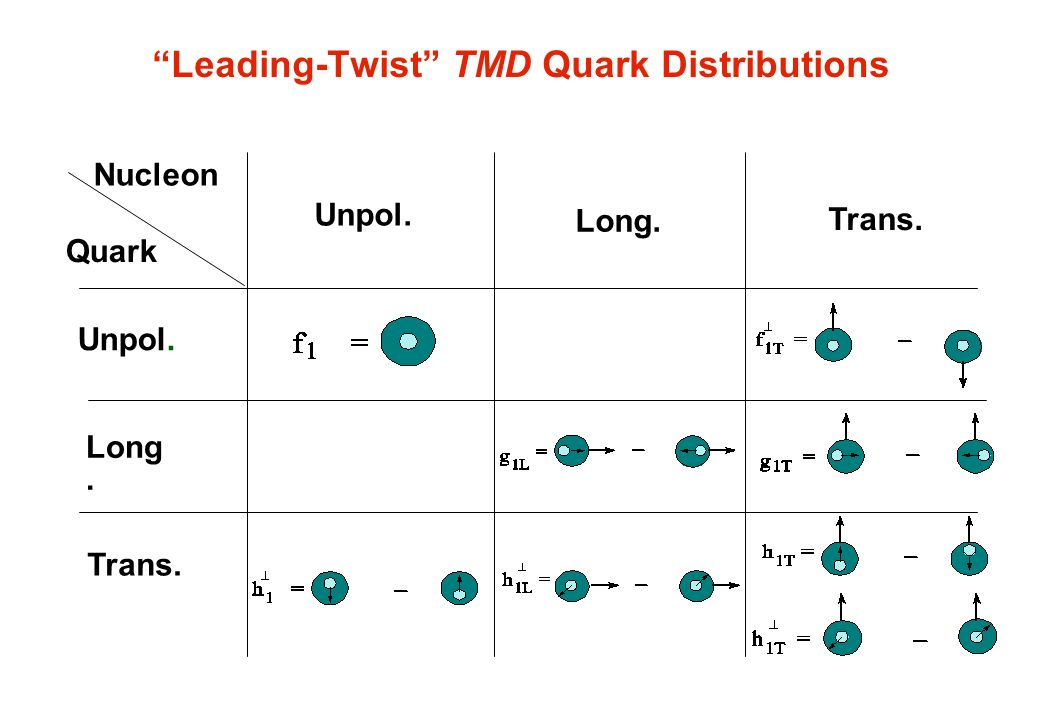
\includegraphics[width = \textwidth]{image/diagrams/tmd-table.jpg}	
%	\caption[Leading order TMD table.]{The twist two TMDs are tabulated in terms of their spin decomposition.}
%	\label{fig:tmd-table}
%\end{figure}
%


\section{This Section Is Not Developed Yet}
In this thesis I present two distinct measurements of SIDIS structure functions and their combinations.  The first observable measured is the unpolarized cross section, which is presented as an extension of the analysis of Nathan Harrison who measured the unnormalized cross sections for charged pions in CLAS [reference to Nate].  Three structure functions appear in this cross section expansion, those which have the unpolarized beam and target subscripts "UU" in the cross section equation.  The leading structure function is not modulated by the phi dependent angle of the outgoing hadron, and is expected to be dominant in size when compared with the two co-sinusoidal structure functions that remain.  This novel measurement compliments the unnormalized work of Nathan Harrison as well as the measurements of multiplicities performed by the HERMES and COMPASS collaborations [reference both of those].  Without applying the TMD framework, this measurement still has value in that it provides the scale of the structure functions for the first time and can be used to predict SIDIS yields for future studies.  Within the TMD framework, the leading order unpolarized structure function is composed of the unpolarized PDF and the unpolarized fragmentation function, both fairly well known from previous experiments.  The phi modulated structure functions contain a TMD PDF known as the Boer-Mulders function, pursued for its possible connection to quark orbital angular momentum.  I expect that the results of this measurement can be used as input, with results from other experiments, to extract the Boer-Mulders TMD using a phenomenological model.

% 9b. BSA 
I also present measurements of positively charged kaon beam spin asymmetries, which addresses several interesting areas of TMD physics.  The beam spin asymmetry, defined as the difference in events observed for different electron helicity states (normalized by the total number of electrons), depends on the observable structure function (F LU SIN PHI).  Interestingly, if one assumes that twist three PDFs and FFs are zero, the beam spin asymmetry term vanishes because the structure function in question is composed of pure twist three products of PDFs and FFs.

% 10. Wes Gohn 
Recently CLAS reported the non-zero BSA measurement of charged and neutral pion beam spin asymmetries, which implies that in the kinematics measured by CLAS, the twist three TMD terms cannot be neglected [reference to Wes Gohn thesis].  As a natural extension of this knowledge, I analyze the same observable for the heavier kaon channel to see if the same conclusion is realized.

% Structural overview of thesis 
I have reviewed the experimental hardware that enables this thesis work in chapter 2 and summarized analytical techniques used during chapter 3.  I describe basic analysis procedures that are common to both measurements in chapter 4 before discussing particle identification in chapter 5.  I present results for the inclusive scattering cross section in chapter 6, followed by the SIDIS cross section in chapter 7.  I then present my findings for the positively charged kaon BSA measurement in chapter 8 before offering a brief summary and outlook in chapter 9. 

%
%  Equations from dissertation proposal 
%
%

\begin{equation}
  e(l) + h(P) \rightarrow e'(l') + h(P_{h}) + X 
\end{equation}

In SIDIS it is customary to define the following kinematic variables (where $q = l - l'$ and $Q^{2} = -q^{2}$). 

\begin{align}
  x = \frac{Q^{2}}{2P \cdot q} && y = \frac{P \cdot q}{P \cdot l} && z = \frac{P \cdot P_{h}}{P \cdot q} && \gamma = \frac{2Mx}{Q}
\end{align}

Additionally, the ratio $\varepsilon$ of the longitudinal and transverse photon flux is shown below.

\begin{equation}
	\varepsilon = \frac{1 - y - \frac{1}{4}\gamma^2 y^2}{1 - y + \frac{1}{2}y^2 + \frac{1}{4}\gamma^2 y^2}
\end{equation}

\begin{eqnarray}
\frac{d\sigma^{e^-P\to e^-hX}}{dx_B \, dy\, d\phi_s \,dz\, d\phi_h\, d p_{h\perp}^2}
&=&\frac{\alpha^2_{em}}{2x_B y Q^2}
\frac{y^2}{1-\varepsilon}  ( 1+\frac{\gamma^2}{2x_B} ) \Bigl\{  \nonumber \\
&& F_{UU ,T} +  \varepsilon F_{UU ,L}
+ \sqrt{2\,\varepsilon (1+\varepsilon)} \cos\phi_h F_{UU}^{\cos\phi_h}
+ \varepsilon \cos(2\phi_h) F_{UU}^{\cos 2\phi_h} \nonumber \\
&+& \lambda_e
\sqrt{2\,\varepsilon (1-\varepsilon)} \sin\phi_h F_{LU}^{\sin\phi_h}
+ \lambda \big[ \sqrt{2 \varepsilon (1+\varepsilon)} \sin\phi_h F_{UL}^{\sin\phi_h}
  +  \varepsilon \sin(2\phi_h) F_{UL}^{\sin 2\phi_h} \big] \nonumber \\
&+&  \lambda_e \lambda
\big[\sqrt{1-\varepsilon^2} F_{LL}
  +\sqrt{2\varepsilon (1-\varepsilon)} \cos\phi_h F_{LL}^{\cos \phi_h}\big] \nonumber \\
&+& s_\perp
\big[ \sin(\phi_h-\phi_S) \bigl(F_{UT ,T}^{\sin(\phi_h -\phi_S)}
  + \varepsilon\, F_{UT ,L}^{\sin(\phi_h -\phi_S)}\bigr) \nonumber \\
  && \phantom{s_\perp}
  + \varepsilon \sin(\phi_h+\phi_S) F_{UT}^{\sin(\phi_h +\phi_S)}
  + \varepsilon \sin(3\phi_h-\phi_S) F_{UT}^{\sin(3\phi_h -\phi_S)} \nonumber \\
  && \phantom{s_\perp}
  + \sqrt{2\,\varepsilon (1+\varepsilon)} \sin\phi_S F_{UT}^{\sin \phi_S }
  + \sqrt{2\,\varepsilon (1+\varepsilon)} \sin(2\phi_h-\phi_S) F_{UT}^{\sin(2\phi_h -\phi_S)}\big]\nonumber \\
&+& \lambda_e s_\perp
\big[\sqrt{1-\varepsilon^2} \cos(\phi_h-\phi_S) F_{LT}^{\cos(\phi_h -\phi_S)}
  +\sqrt{2\varepsilon (1-\varepsilon)} \cos\phi_S F_{LT}^{\cos \phi_S} \nonumber \\
  && \phantom{\lambda_e s_\perp}
  +\sqrt{2\,\varepsilon (1-\varepsilon)} \cos(2\phi_h-\phi_S) F_{LT}^{\cos(2\phi_h - \phi_S)} \big] \Bigr\},
\label{e:crossmaster}
\end{eqnarray}


Here $\lambda_e$ refers to the helicity of the incoming lepton (beam electron in our case).  If one decomposes the hadronic matrix element which is present in the hadronic tensor into different possible Dirac structures, a set of functions known as transverse momentum dependent parton distributions functions (TMD PDFs) and transverse momentum dependent fragmentation functions (TMD FFs) can be defined.  The structure functions from above can then be calculated as a convolution of these more basic non-perturbative functions.  The notation $\mathcal{C}$ is shorhtand  presented in \cite{tmds-bacchetta:2006} as a way to write structure functions in terms of the convolutions of PDF and FF objects.

\begin{equation}
  \mathcal{C}[\omega f D] = x \sum_{a} e^{2}_{a} \int d^{2}\pt d^{2}\kt \delta^{(2)} \left( z\kt + \pt - \vect{P}_{h\perp} \right) \omega (\kt, \pt) f^{a}(x, k_{T}^{2}) D^{a}(z, p_{T}^{2}) 
\end{equation}

where a is summed over quarks and anti-quarks.  The five structure functions appearing in the cross section are, 

\begin{equation}
F_{UU,T} = \mathcal{C}[f_1 D_1] = x \sum_{a} e^{2}_{a} \int d^{2} \pt d^{2} \kt \delta^{(2)} \left( z\kt + \pt - \vect{P}_{h\perp} \right) f_{1}^{a}(x, k_{T}^{2}) D_{1}^{a}(z, p_{T}^{2})
\end{equation}

\begin{equation}
F_{UU,L} = 0
\end{equation}

\begin{equation}
F_{UU}^{\cos \phi_h} = \frac{2M}{Q} \mathcal{C}[ - \frac{\hhat \cdot \kt}{M_h} \Bigl( x h H_{1}^{\perp} + \frac{M_h}{M} f_1 \frac{\tilde{D}^{\perp}}{z} \Bigr) - \frac{\hhat \cdot \pt}{M} \Bigl( x f^{\perp} D_1 + \frac{M_h}{M} h_1^{\perp} \frac{\tilde{H}}{z} \Bigr)]
\end{equation}

\begin{equation}
F_{UU}^{\cos 2\phi_h} = \mathcal{C}[- \frac{2 (\vect{\hat{h}} \cdot \kt) (\vect{\hat{h}} \cdot \pt) - \kt \cdot \pt}{M M_h} h_{1}^{\perp} H_{1}^{\perp} ]
\end{equation}

\begin{equation}
  F_{LU}^{\sin\phi} = \frac{2M}{Q} \mathcal{C} \Bigl[ -\frac{\hhat \cdot \kt}{M_h} \Bigl( xeH_1^\perp + \frac{M_h}{M} f_1 \frac{\tilde{G}^\perp}{z} \Bigr) + \frac{\hhat \cdot \pt}{M} \Bigl( xg^\perp D_1 + \frac{M_h}{M} h_{1}^{\perp} \frac{\tilde{E}}{z} \Bigr) \Bigr]
\end{equation}

\begin{equation}
  BSA = \frac{d\sigma^+ - d\sigma^-}{d\sigma^+ + d\sigma^-} = \frac{\phimod{LU}{\sin\phi}}{1 + \phimod{UU}{\cos\phi} + \phimod{UU}{\cos(2\phi)}}
\end{equation}

Where the coefficient $A_{LU}^{\sin\phi}$ is defined as, 

\begin{equation}
  A_{LU}^{\sin\phi} = \sqrt{2\,\varepsilon (1-\varepsilon)} \frac{F_{LU}^{\sin\phi}}{F_{UU,T} + \varepsilon F_{UU,L}}
\end{equation}
